\documentclass{jsarticle}
\usepackage[top=20truemm,bottom=20truemm,left=25truemm,right=25truemm]{geometry}
\usepackage{amsmath,ascmac,url,amsfonts,bm,here,algorithmic,algorithm,amsthm,color}
\usepackage[dvipdfmx]{graphicx}
\newcommand{\argmax}{\mathop{\rm argmax}\limits}
\newcommand{\argmin}{\mathop{\rm argmin}\limits} 
\newcommand{\expect}{\mathbb{E}} 
\newcommand{\trans}[1]{#1^{\top}}
\newcommand{\pdif}[2]{\frac{\partial#1}{\partial#2}}
\newcommand{\odif}[2]{\frac{\rm{d}#1}{\rm{d}#2}}
\makeatletter
  \def\@maketitle{
  \newpage\null
  \vskip 2em
    \mbox{}\hfill
    \begin{flushleft}
    \textbf{制御システム論分野研究会資料}
    \end{flushleft}
    \begin{flushright}
    {\lineskip .5em
      \begin{tabular}[t]{c}
        \@date \\
        \@author
      \end{tabular}\par}
        \end{flushright}
  \begin{center}
  \let\footnote\thanks
    {\LARGE \@title \par}
    \vskip 1.5em
  \end{center}
    \vskip 1em
  \par}
\makeatother
\title{\large{\bf{進捗報告 10.1}}}
\author{M2 竹内 維吹}
\date{\today}
\begin{document}
\maketitle


\section{前提}
入力アフィン系のセルフトリガー制御を考える. 
\begin{equation}
	\dot{s} = f(s) + g(s)a \label{continuous}
\end{equation}

\subsection{倒立振子による実験}
倒立時の振子の角度を$\theta=0$とし, 加えられる入力が$A=[-10\textrm{N}\cdot\textrm{m},10\textrm{N}\cdot\textrm{m}]$と制限されるような倒立振子を考える.この倒立振子のダイナミクスは, 以下のように与えられる.
\begin{equation}
	\odif{}{t}\begin{pmatrix}\theta \\ \dot{\theta}\end{pmatrix} = 
		\begin{pmatrix}\dot{\theta} \\ \frac{3g}{2l}\sin{\theta} + \frac{3}{ml^2}a \end{pmatrix} \label{pendulum}
\end{equation}

コンピュータで強化学習を行う場合, これを離散化したシステムについて計算を行う必要がある.上記の状態方程式を離散化すると以下のようになる.
\begin{align}
	\theta_{t+1} &= \theta_t+\dot{\theta}_t\delta_t+\frac{3g}{2l}\sin{\theta_t}\delta_t^2+\frac{3}{ml^2}a\delta_t^2 \tag{3a}\\
	\dot{\theta}_{t+1} &=  \dot{\theta}_t+\frac{3g}{2l}\sin{\theta_t}\delta_t+\frac{3}{ml^2}a\delta_t \tag{3b}
\end{align}\label{pend}
\setcounter{equation}{3}
ただし, $\delta_t$は離散化定数である.\par


\section{現状確認}
\subsection{セルフトリガー制御}
図\ref{image}のような制御系を考える.
\begin{figure}[h]
	\centering
 	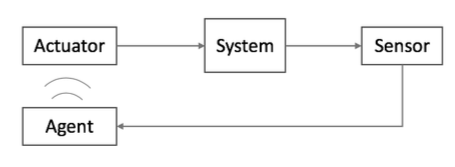
\includegraphics[width=10cm]{event.png}
 	\caption{制御系} \label{image}
\end{figure}\par
これに対するフィードバック制御を考える. 状態変数$s$を観測してアクチュエータに入力信号を送信することを「インタラクション」と呼ぶと,セルフトリガー制御では, 連続的なインタラクションは行わずに, 次のインタラクションを何秒後に行うかをエージェントが決定する. それを数式上で表すため, エージェントの制御則$\pi(s)$は2つの要素からなるベクトル値関数であるとし, 1つ目の要素はアクチュエータに送信する入力$a$,~2つ目の要素は次にインタラクションを行うまでの時間間隔$\tau~(s:秒)$を表すものとする.また, 次のインタラクションを行う時刻までは1つ前のインタラクションで送信した入力$a$を加え続けるものとする(ZOH制御).

\subsection{目標点の確認}
研究を通しての目標は「安全性を確保しながら, 最適セルフトリガー制御則$\pi^{*}$の強化学習を実現させること」である。ここで
\begin{align}
	\pi^{*} &= \argmax_{\pi}J(\pi) \label{optimal_policy}\\
	J(\pi) &= \expect_{s_0\in d_0}[V^{\pi}(s_0)] \\
	% V^{\pi}(s_0) &= \sum_{i=0}^{\infty} \gamma^i\{-s_i^{\top}Qs_i-\pi_1(s_i)^{\top}R\pi_1(s_i)+\lambda \pi_2(s_i)\} \\
	V^{\pi}(s_0) &= \sum_{i=0}^{\infty} \gamma^i C^{\pi}_i \label{value} \\
	C^{\pi}_i &= -\int_{T_i}^{T_{i+1}}s(t)^{\top}Qs(t)\textrm{d}t +\tau_ia_i^{\top}Ra_i + \lambda \tau_i, ~T_i = \sum_{l=0}^{i} \tau_l \label{reward}
\end{align}
であり,~$\pi_1, \pi_2$は$\pi$の第1,第2成分である. また, $i$はインタラクションの回数を示し, $a_i, \tau_i$はそれぞれ$i$回目のインタラクションでの方策$\pi$の出力である. \par
さて, 一般的に強化学習では, 1ステップ1ステップの行動の良し悪しを評価して方策を更新していく. 
インタラクションとインタラクションの間の区間を「インターバル」と呼ぶと, 式(\ref{value})より, この問題は各インターバルを1ステップとした強化学習問題であると考えることができる. \par
以下では方策$\pi$を$\theta$でパラメトライズし, $\theta^{*} = \argmax_{\theta}J(\pi_{\theta})$を解くことによって$\pi^{*} = \argmax_{\pi}J(\pi)$を得るものとする. 方策勾配を用いた強化学習では$\nabla_{\theta}J(\pi)$を用いて$\theta^{*}$を求める. その際方策勾配$\nabla_{\theta}J(\pi)$の近似のため, 実環境とのインタラクションによって得られたデータ組$\{s,a,r,s^{\prime}\}$を用いる. 「学習中の安全」という言葉を, 「このデータ組の収集を決められた安全領域$\mathcal{C}$の内部でのみ行うこと」と定義する.\par


\subsection{実現可能性の検証:サンプル値系での実験}
上記の目標を達成する見込みがあるのかを検証するために, サンプル値系での実験を行う. サンプル値系では,セルフトリガー制御と同様に連続的なインタラクションは行わない. セルフトリガー制御との違いは, インタラクションの間隔がエージェントによって状態$s$依存で決定するのではなく, 制御問題の設定として定数$t_{\rm{int}}$で与えられる点である.したがってサンプル値系での制御方策$\pi_{\rm{sample}}$は,アクチュエータに送信する入力信号$a$のみを出力する関数として与える.\par
サンプル値系での実験により, $t_{\rm{int}}=0.001(s)$のサンプル値系での最適方策
\begin{align}
\begin{cases}
	\pi_{\rm{sample},1} = -\argmax_{\pi_{\rm{sample}}} \displaystyle\sum_{i=0}^{\infty} \int_{it_{\rm{int}}}^{(i+1)t_{\rm{int}}}s(t)^{\top}Qs(t)\textrm{d}t + t_{\rm{int}}a_i^{\top}Ra_i \\
	a_i  = \pi_{\rm{sample}}(s(it_{\rm{int}}))
\end{cases}
\end{align}
を初期方策として,~$t_{\rm{int}}=0.002(s)$のサンプル値系での最適方策
\begin{align}
\begin{cases}
	\pi_{\rm{sample},2} = -\argmax_{\pi_{\rm{sample}}} \displaystyle\sum_{i=0}^{\infty} \int_{it_{\rm{int}}}^{(i+1)t_{\rm{int}}}s(t)^{\top}Qs(t)\textrm{d}t + t_{\rm{int}}a_i^{\top}Ra_i  \\
	a_i  = \pi_{\rm{sample}}(s(it_{\rm{int}}))
\end{cases}
\end{align}
 を学習中の安全性を満たしながら学習できるかを検証する. 

\subsection{セルフトリガー制御への発展}
前節での検証によって, インタラクション間隔を大きくしても安全強化学習を行うことが可能であることを確認できたとする. サンプル値系での制御則は入力信号$a$のみを出力する関数であったので, 入力信号$a$とインタラクション間隔$\tau$の二つの要素を出力する必要があるセルフトリガー制御の初期方策として方策$\pi_{\rm{sample},1}$をそのまま用いることはできない. \par
そこで代替策として,
\begin{align}
\begin{cases}
	\pi_1(s)=\pi_{\rm{sample},1}(s)\\
	\pi_2(s)=0.001
\end{cases} \label{pi_init}
\end{align}
とする方策$\pi_{\rm{init}}$をセルフトリガー制御の強化学習のための初期方策として用いる.

\section{安全性の定義}
\subsection{インタラクション間隔$\tau$の安全性}
ECBF(後から書きます)


\subsection{入力信号$a$の安全性}
強化学習ではデータの収集に環境とのインタラクションを行う必要がある. DDPGと呼ばれるアルゴリズムは方策オン型の強化学習とよばれ, データの収集方策に学習中の暫定最適方策を用いる. したがって,学習初期の方策では安全性が保証されないことがしばしばある. この課題を解決するために, 制御バリア関数を用いる. \par
関数$h(s)$が以下の条件を満たす時, システム(\ref{continuous})に対する制御バリア関数であるという. 
\begin{equation}
	\sup_{a\in A}\left\{\pdif{h}{s}(f(s)+g(s)a)+K(h(s))\right\} \geq 0 \label{CBF}
\end{equation}
ただし, $K(s)$はクラスK関数である.\par
さて, 2.2節にて登場した安全領域$\mathcal{C}$を
\begin{equation}
	\mathcal{C} = \left\{s \in S~|~h(s)\geq 0\right\}
\end{equation}
として与える. このとき$h(s)$が制御バリア関数であるならば, 状態$s\in C$を初期状態とした時, それ以降の全時刻において, 状態$s$が$s\in C$を満たすようにする入力が存在することを保証する. そのような入力集合は現時刻での状態$s$に依存し,
\begin{equation}
	U(s) = \left\{a \in A~|~\pdif{h}{s}(f(s)+g(s)a)+K(h(s))\geq 0\right\}, \forall s\in C
\end{equation}
としてその集合を与える.\par
学習中の安全性を確保するために, 図2のようにエージェントの出力を$U(s)$の要素に射影するレイヤーを設ける.
\begin{figure}[h]
	\centering
 	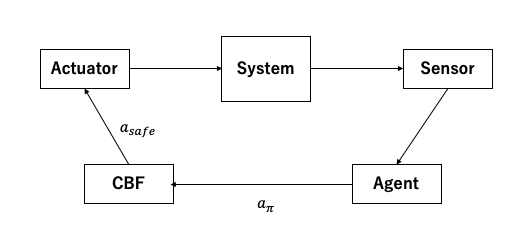
\includegraphics[width=10cm]{barrier_certificate.png}
 	\caption{制御系} \label{cbf}
\end{figure}\\
当面は, エージェントの出力$a_{\pi}$に最も近い$U(s)$の元への射影を考える.



\section{今後の方針}
\subsection{シミュレーション環境の構築}
さて, 制御バリア関数による安全性保証は連続システムに対して行われるものである. また, セルフトリガー制御則の第2成分$\tau$の出力ロジックを勾配によって更新できるように, $\tau$を連続値として扱う必要がある. しかし, コンピュータ上でシミュレーションを行うには(\ref{continuous})を時間に関して離散化を行わなくてはならない.\par
そこで, インタラクション間隔$\tau$を整数個に等間隔に分割し, その時間幅を用いて離散化を行う. この時, 離散化幅は$0.001(s)\sim 0.005(s)$になるように分割数を調整する. $\delta_t$を上から抑える理由は離散化誤差を抑えるためである. ($\tau$を)下から抑えるのは,コンピュータ上で$\frac{1}{\infty}=0$となってしまうからで, それを回避するためである.\par
ここで, 式(\ref{reward})のインターバル報酬$C^{\pi}_i$が定積分を用いて表されているため, これをシミュレーション環境で近似する手法を考える. ダイナミクス(\ref{continuous})の離散化幅$\delta_t$の離散近似システムが
\begin{equation}
	s_{t+1} = f_d(s_t, \delta_t) + g_d(s_t, \delta_t)a_t
\end{equation}
と書かれているとする. インタラクション間隔$\tau$を$N$分割した時, $\delta_t = \frac{\tau}{N}$を用いて
\begin{equation}
	C^{\pi}_i \approx -\delta_t\sum_{k=0}^{N}s_{n_i+k}^{\top}Qs_{n_i+k}+\tau_ia_i^{\top}Ra_i + \lambda \tau_i
\end{equation}
と近似する. ここで$s_{n_i}$は$i$回目のインタラクションを行った瞬間の状態変数$s(T_i)$と同じ値が代入されるものとする.\par

\subsection{サンプル値系での安全性確保ロジックの構築}
2.3節で記述した通り, $t_{\textrm{int}}$が$0.001(s)$の最適方策$\pi_{\textrm{sample},1}$を初期値として,~$0.002(s)$の最適方策$\pi_{\textrm{sample},2}$を安全強化学習できるのか検証する. 本節ではその安全性の確保方法についてもう少し掘り下げて議論する.\par
ECBFを用いることによって, 入力$a$に対するインタラクション間隔$\tau$の限界を与えることができる. その値を$\tau_{\textrm{max}}(a)$と書く. もし$\tau_{\textrm{max}}(a)<0.002$であるなら, CBFを用いて$U(s)$の元$a_{\textrm{safe}}$を選び$\tau_{\textrm{max}}(a_{\textrm{safe}})\geq0.002$となれば, 次のインタラクションまで$a_{\textrm{safe}}$を加え続けても状態変数が$\mathcal{C}$を出ていくことはない.しかし$\forall a \in U(s)$に対して$\tau_{\textrm{max}}(a)<0.002$であるなら, 次のインタラクションを$0.001(s)$後に行うことで, 安全性を確保する必要がある. ~($0.001\leq\tau_{\textrm{max}}(a)<0.002$を仮定)\par
ここまでの議論を整理すると, 「サンプル値系における安全性保証」とは「1. 入力信号の安全性,~2. サンプル間隔の安全性」を保証することになる. これらが行われることを回避する学習方法については今後検討する.


\subsection{セルフトリガー制御の強化学習}
2.4節で記した初期方策$\pi_{\rm{init}}$から, 安全性を保証しながら最適セルフトリガー制御則$\pi^{*}$の学習を試みる. サンプル値系とは異なり, インタラクション間隔はエージェントが決定する. したがって, 方策関数の出力$\pi(s) = \begin{bmatrix}a & \tau\end{bmatrix}$に対して,~$\tau>\tau_{\textrm{max}}(a)$となった時には入力信号$a$を変更する方法と, 通信間隔$\tau$を変更する方法の二種類の選択があり, どちらを行うべきか考える必要がある.


\section{(先行して) セルフトリガー制御の強化学習の実験}
現状, ECBFについてまだ深い考察と実装を行っていないので, セルフトリガー制御の安全性の確保は行うことはできない.しかしながら$\pi_{\textrm{init}}$から$\pi^{*}$を強化学習するための環境は整っているため, 安全性については考慮せずに実験を行ってみた.\par
実験環境はOpen-AI Gymのpendulumで, 初期状態が$\theta\sim N(0, 0.1), \dot{\theta}\sim U(-1,1)$となるような環境で行った. また, 10秒間の制御を1エピソードと定義する.\par

\subsection{$\lambda$による学習過程の変化}
式\eqref{reward}より, $\tau$を大きくするモチベーションは$\lambda$に大きく依存するため, それを様々な値にすることでど学習過程にどのような変化が見られるのかを確認してみた. ここでは,~$\lambda$を$0.05, 0.5, 5, 50$に設定し, それぞれ3回, 200000ステップ(インタラクションの回数)の強化学習を行った. また,~$\tau$は$0.001\sim0.1$の範囲に制限している.\par
まずそれぞれの学習タスクの中で, 1エピソードの間の$\tau$の平均値の変化を見てみる.\par
\begin{figure}[h]
	\centering
 	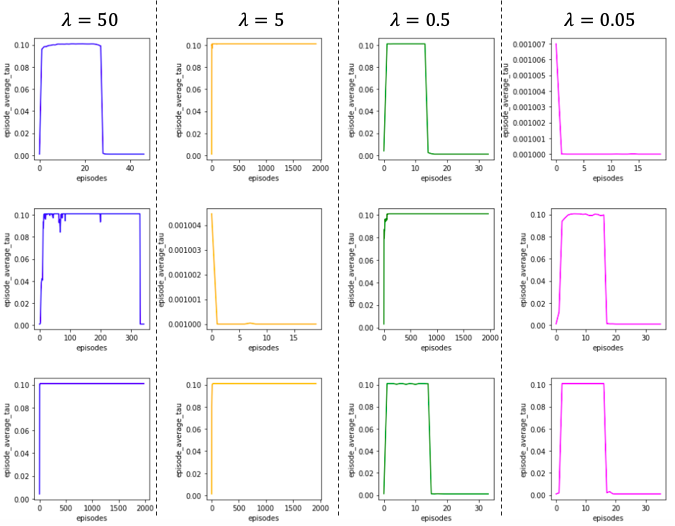
\includegraphics[width=14cm]{tau_exp_ave.png}
 	\caption{学習を通しての$\tau$の変化} \label{average_tau}
\end{figure}
ここで注意したいのは, $\tau$によって200000回のインタラクションに含まれるエピソード数が異なる点である. 例えば$\tau$の学習が進まずにずっと$\tau=0.001$であった場合, 10秒間の制御の間には10000回のインタラクションが行われる. したがって200000回のインタラクションの間には20エピソードしか含まれない. 逆に, 初期から$\tau$の学習が進み$\tau=0.1$となることが増えてくると, エピソード数は増えてくる. 図\ref{average_tau}の$x$軸の範囲が異なるのはそのためである. \par
次に, 制御性能(倒立振子の制御)の変化を見るためこの時のそれぞれのエピソード報酬の変化を見てみる. 
\begin{figure}[h]
	\centering
 	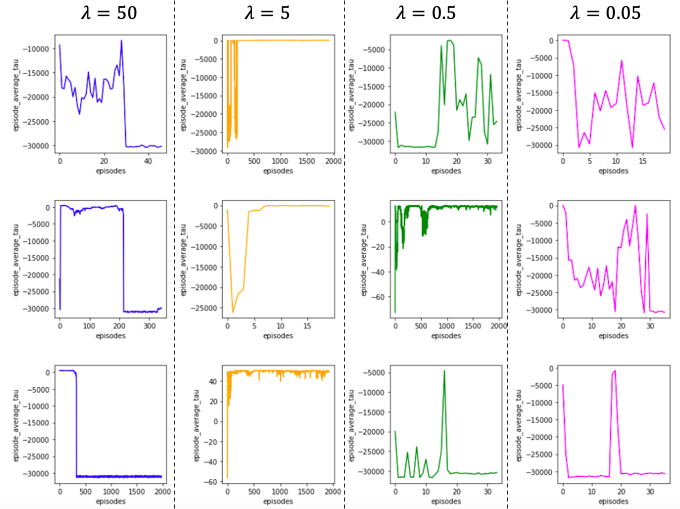
\includegraphics[width=14cm]{reward_log.png}
 	\caption{学習を通してのエピソード報酬の変化} \label{reward_log}
\end{figure}\\

\subsection{考察}
図\ref{reward_log}の各ブロックが表す学習の記録は図\ref{average_tau}と対応している. これら2つの図を見比べてみるといくつかの点に気付く.
\begin{enumerate}
  \item $\lambda=0.1$を初期に学習できていないと, 最終的に得られる制御性能自体も悪化する.
  \item $\lambda$が大きい方が$\tau$を大きくする方向に学習が進みやすい(当然)が, 毎回そうなる訳でもない点
  \item $\lambda=0.1$を学習できていても, $\lambda=0.001$に逆戻りしてしまうことがある. 
\end{enumerate}
1. について,rewardの改善が見られないのはエピソード数が少ないためであることは予想がつくが, ~$\pi_{\textrm{init}}$は$\tau=0.001$において, 原点付近で線形化したシステムを安定化する方策であるため, rewardが減っていくことは腑に落ちない.\\
3. については, rewardをみると$\tau=0.1$を維持している学習とそうでない学習で, $\tau=0.1$の間の制御性能に差がある点ことがわかり, これが理由だと考える. ただし, $\lambda=50$の学習での逆行は理由がわからない.\par

\section{学習した方策による制御性能}
図\ref{average_tau},図\ref{reward_log}を見ると, 勾配法が収束してるとは結論づけられない.この課題が生じている原因として, パラメータ更新に用いる勾配法の学習率が大きすぎるというものが考えられる.\par
しかしながら$\tau(s)$は図\ref{actor_NN}のように$\pi(s)$を表現するニューラルネットワークの出力の1つとして与えているので, $\tau(s)$の学習率のみを小さくすることはできない(入力信号$a(s)$の学習も遅くなってしまう).
\begin{figure}[h]
	\centering
 	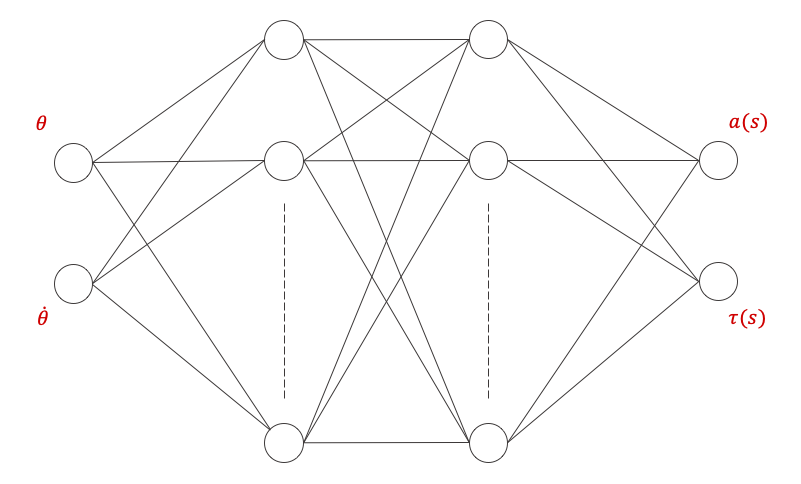
\includegraphics[width=10cm]{actor_NN.png}
 	\caption{方策$\pi_{\theta}(s)$}  \label{actor_NN}
\end{figure}\\
そこで図\ref{split_NN}のようにニューラルネットワークを分離して, $a(s)と\tau(s)$をそれぞれ別のニューラルネットワークで表現する.
\begin{figure}[h]
	\centering
 	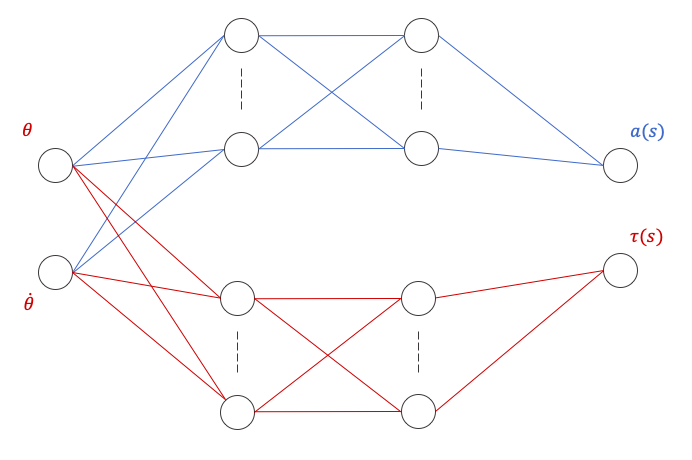
\includegraphics[width=10cm]{split_NN.png}
 	\caption{方策$\pi_{\theta}(s)$の分離}  \label{split_NN}
\end{figure}\\
こうすることで,入力信号$a(s)$とインタラクション間隔$\tau(s)$の学習率を別々にすることができる.\par

\subsection{学習率}
さて, 少し話題が変わるが使用しているDDPGというアルゴリズムでは, actor,criticと二つのNNを用いる. そのうち方策$\pi(s)$はactorのNNによって表される. actorは方策勾配$\nabla_{\theta^{\mu}}J(\pi_{\theta^{\mu}})$によって以下のように更新される.
\begin{equation}
	\theta_{\mu} \gets \theta_{\mu}+ \alpha l_{\textrm{algo}}\circ\nabla_{\theta^{\mu}}J(\pi_{\theta^{\mu}}) \label{policy_update}
\end{equation}
ただし, $\alpha$は固定パラメータで$l_{\textrm{algo}}$は最適化アルゴリズムによってミニバッチに適応して算出されるベクトルであり,~$\nabla_{\theta^{\mu}}J(\pi_{\theta^{\mu}})$にエレメントワイズにかかる. ここでいう最適化アルゴリズムとはSGD, adamなどである. 前節で自由に設定できるとした学習率とは$\alpha$のことであるため, 前節のNN分離は$\tau(s)$の学習率を押さえ込んでいるとは言えない. (adamによって算出される$l_{\textrm{algo}}$については次週調べたい.)また, $\theta_{\mu}$はactorのパラメータを表す.\par
actorのNNを分離したことにより, 式\eqref{policy_update}を
\begin{align}
\theta_{\mu} = \begin{bmatrix}\theta_a \\ \theta_{\tau}\end{bmatrix}, 
\begin{cases}
	\theta_a \gets \theta_a+ \alpha_a l_{\textrm{algo},a}\circ\nabla_{\theta_a}J(\pi_{\theta^{\mu}})|_{\theta_{\tau}} \\
	\theta_{\tau} \gets \theta_{\tau}+ \alpha_{\tau} l_{\textrm{algo},\tau}\circ\nabla_{\theta_{\tau}}J(\pi_{\theta^{\tau}})|_{\theta_a}
\end{cases}
\end{align}
のように分離することができる.

\subsection{学習進捗の確認}
図\ref{reward_log}のように, 1エピソード(10sの制御)の間の報酬を計算したのでは式\eqref{optimal_policy}に対する学習の進捗ができているかは真に確認することができない. そこでDDPGが方策勾配を用いた手法であることから, 学習の進捗を方策勾配のノルムの変化によって確認する(勾配法が収束しているならノルムが0になるはずである).図\ref{gradient_log}に$\alpha_{a}=0.001, \alpha_{\tau}=0.0001$として最適化アルゴリズムにadamを用いた学習の様子を示す.
\begin{figure}[h]
	\centering
 	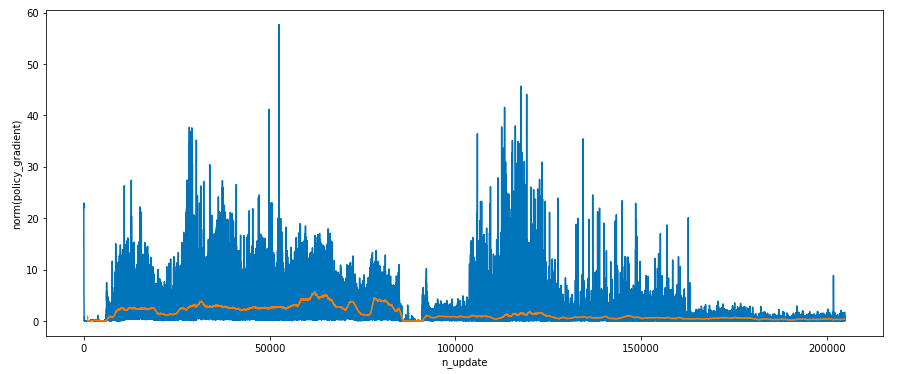
\includegraphics[width=15cm]{gradient_log.png}
 	\caption{学習中の$\|\nabla_{\theta^{\mu}}J(\pi_{\theta^{\mu}})\|_{L_2}$の変化}  \label{gradient_log}
\end{figure}\\
図\ref{gradient_log}はパラメータの更新に用いるための方策勾配$\nabla_{\theta^{\mu}}J(\pi_{\theta^{\mu}})$のL2ノルムの変化をプロットしている. オレンジ線は1000ステップの移動平均線である.図\ref{gradient_log}を見ると方策勾配が収束しているとは結論づけにくい.
\par
比較対象として, セルフトリガーやイベントトリガーなどが一切関係ない「プレーンな」倒立振子の「振り上げ」の強化学習における方策勾配もみてみた.
\begin{figure}[h]
	\centering
 	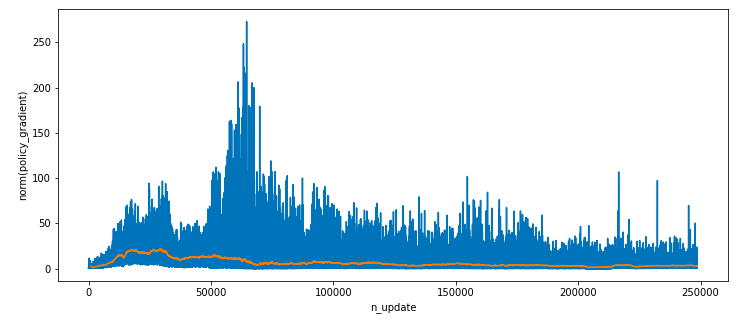
\includegraphics[width=16cm]{gradient_log_plain.png}
 	\caption{比較: プレーンな倒立振子の学習}  \label{gradient_log_plain}
\end{figure}\\
この学習はまだ決して収束しているとは言えないが, 移動平均線を見ると概ね単調減少していることから, 着実に学習が進んでいると考えられる. 

\subsection{考察}
前節で, セルフトリガー強化学習の方策勾配のL2ノルムが収束できていない様子を確認した. この原因について考察する.\par
DDPGがそのアルゴリズムの根底として用いているのは以下の方策勾配定理である.
\begin{equation}
	\nabla_{\theta}J(\pi_{\theta}) = \expect_{\pi_{\theta}}[\nabla_{\theta}\log\pi_{\theta}(s)Q^{\pi}(s,a)]
\end{equation}
しかしながら, DDPGでは$Q^{\pi}(s,a)$をcriticのNNが関数近似しているため, 計算している方策勾配は近似方策勾配となり, イメージ通りの勾配のノルムの単調減少が見られていないのではないかと考える. 逆に言えば, 勾配法が正しく進んでいない理由が$\tau$の学習率以前に, criticの学習がまだ不十分であることが原因だとわかったので, より多くの学習時間が必要であると考えられる.(やります)


\begin{thebibliography}{10}
\bibitem{ECBF}
G. Yang, C. Belta, and R. Tron. “Self-triggered Control for Safety Critical Systems Using Control Barrier Functions."  \textit{In American Control Conference (ACC) Philadelphia, USA}, 2019.
 
 \end{thebibliography}
\end{document}